\atsp
\begin{frame}{\ft{Obtaining Information About Parameters}}
\section{Group 1: Obtaining Information About Parameters}

	\pdfpageheight 30cm

        \begin{annotatedFigure}{0pt}{0pt}
            {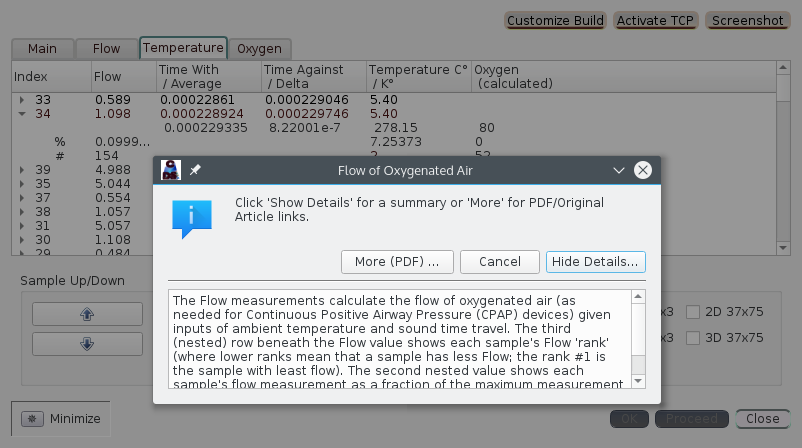
\includegraphics[scale=1.5]{texs/about.png}}
            
\pgfdeclareverticalshading{myshading}{100bp}{color(0bp)=(yellow!60); 
	%color(30bp)=(yellow!10); 
	%color(70bp)=(green!10); 
	color(100bp)=(green!10)}
            
  \node [text width=13cm,inner sep=14pt,align=justify,%fill=logoCyan!20, %draw=logoBlue, 
  %draw opacity=0.5,
  line width=1mm, fill opacity=0.9,
  draw=green!40!black,shading=myshading, 
  shading angle=125]
   at (0.58,0.76){\annfont\textbf{Context menus also allow users to 
   obtain information and explanations about individual parts of the 
   data set, such as individual statistical parameters.  In this 
   screenshot, the user has right-clicked on a data column (Flow) and 
   has chosen a context menu action which shows, via a dialog box, 
   a precis of the quantities represented in that column and their 
   significance for the data set as a whole.}};

            \annotatedFigureBox{0.2,0.12}{0.812,0.645}{1}{0.81,0.645}%       
        \end{annotatedFigure}

\end{frame}
